\begin{lstlisting}
第4章:14 17 18 19 
第5章:1 2 3 7
\end{lstlisting}
\begin{exercise}
\begin{figure}[H]
\centering
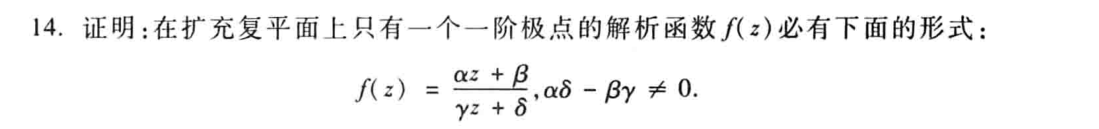
\includegraphics[width=\textwidth]{hw9-2025042910.png}
% \caption{}
\label{}
\end{figure}
\end{exercise}
\begin{proof}
\[
f(z)=c_{-1}(z-z_0)^{-1}+c_0+\sum_{n=1}^{\infty} c_n(z-z_0)^{n}
\]
Since $f\in H(\overline{\mathbb{C}})$,
\[
f\left( \frac{1}{z} \right)=c_{-1} \frac{z}{1-z_0z}+c_0+\sum_{n=1}^{\infty} c_n(z^{-1}-z_0)^{n}
\]
is holomorphic at $z=0$. Thus $c_n=0,\forall n\geq1$.
\[
f(z)=\frac{c_{-1}}{z-z_0}+c_0=\frac{c_0z-c_0z_0+c_{-1}}{z-z_0}
\]
where
\[
\alpha=c_0 ,\quad \beta=-c_0z_0+c_{-1},\quad \gamma=1,\quad \delta=-z_0
\]
And $\alpha\delta-\beta\gamma\neq0$.
\end{proof}

\begin{exercise}
\begin{figure}[H]
\centering
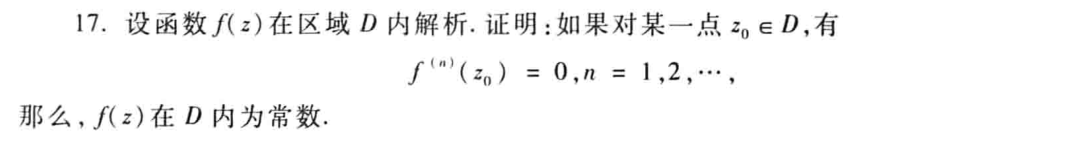
\includegraphics[width=\textwidth]{1-hw9-2025042910.png}
% \caption{}
\label{}
\end{figure}
\end{exercise}
\begin{proof}
For $z\in D$, we have
\[
f(z)=\sum_{n=0}^{\infty} c_n(z-z_0)^{n}
\]
where $c_n=\frac{f^{(n)}(z_0)}{n!}$. Since $f^{(n)}(z_0)=0$ for $n=1,2,\dots$. Then $c_n=0$ for $n=1,2,\dots$. Therefore
\[
f(z)\equiv c_0
\]
is constant in $D$.

\end{proof}

\begin{exercise}
\begin{figure}[H]
\centering
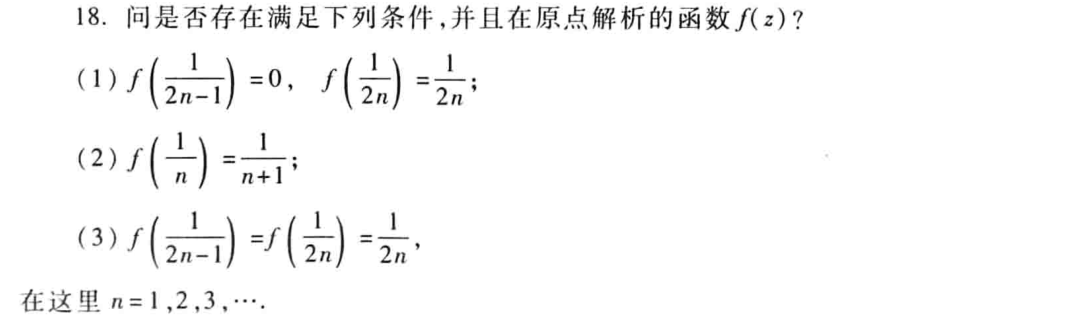
\includegraphics[width=\textwidth]{2-hw9-2025042910.png}
% \caption{}
\label{}
\end{figure}
\end{exercise}
\begin{proof}
(1)
不存在,由于非平凡解析函数零点孤立,而 $\left\{  \frac{1}{2n-1}  \right\}\to0$, $f$ 在 0 的某个邻域内恒为 0. 当 $n$ 充分大的时候 $\frac{1}{2n}$ 落在这个邻域内,但 $f\left( \frac{1}{2n} \right)=\frac{1}{2n}\neq0$.

(2)
可做函数
\[
f(z)=\frac{z}{z+1}
\]
(3)
不存在,事实上点列 $\left\{  \frac{1}{2n}  \right\}\to0$,故在 0 的某个邻域内, $f(z)-z\equiv0$,这与题设 $f\left( \frac{1}{2n-1} \right)=\frac{1}{2n}$ 矛盾.

\end{proof}

\begin{exercise}
\begin{figure}[H]
\centering

\includegraphics[width=\textwidth]{3-hw9-2025042910.png}
% \caption{}
\label{}
\end{figure}
\end{exercise}
\begin{proof}
并不矛盾,因为 1 是函数的奇点,函数不在 1 处解析.

\end{proof}

\begin{exercise}
\begin{figure}[H]
\centering
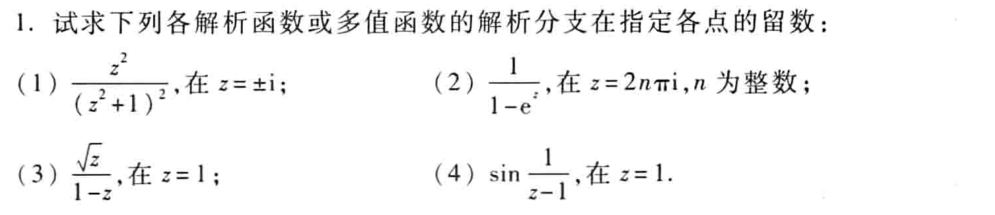
\includegraphics[width=\textwidth]{4-hw9-2025042910.png}
% \caption{}
\label{}
\end{figure}
\end{exercise}
(1)
\[
\begin{aligned}
\mathrm{res}_{i}\frac{z^2}{(z^2+1)^2} & =\frac{1}{1!}\cdot \lim_{ z \to i } \frac{\mathrm{d}}{\mathrm{d}z} \left[ (z-i)^{2}\frac{z^2}{(z-i)^2(z+i)^2} \right] \\
 & =\lim_{ z \to i } \frac{z^2}{(z+i)^2} \\
 & =\frac{1}{4}
\end{aligned}
\]
\[
\begin{aligned}
\mathrm{res}_{-i}\frac{z^2}{(z^2+1)^2} & =\frac{1}{1!}\cdot \lim_{ z \to -i}\frac{\mathrm{d}}{\mathrm{d}z} \left[ (z+i)^2\frac{z^2}{(z-i)^2(z+i)^2} \right] \\
 & =\lim_{ z \to -i } \frac{z^2}{(z-i)^2} \\
 & =\frac{1}{4}
\end{aligned}
\]
(2)
\[
\mathrm{res}_{2n\pi i}\left( \frac{1}{1-e^{ z }} \right)=\lim_{ z \to 2n \pi i } \frac{z-2n\pi i}{1-e^{ z }}=-1
\]
(3)
\[
\mathrm{res}_{1}\left( \frac{\sqrt{ z }}{1-z} \right)=1
\]
(4)
\[
\mathrm{res}_{1}\left( \sin\frac{1}{z-1} \right)=\lim_{ z \to 1 } (z-1)\sin\frac{1}{z-1}=1
\]
\begin{exercise}
\begin{figure}[H]
\centering

\includegraphics[width=\textwidth]{5-hw9-2025042910.png}
% \caption{}
\label{}
\end{figure}
\end{exercise}
\[
\frac{\mathrm{Ln}z}{z^2-1}=\frac{\ln \lvert z \rvert+i\arg z +2n\pi i}{(z-1)(z+1)}\eqqcolon f(z)
\]
$n=0$ 时,$f(z)$ 在 $z=1$ 处有可去奇点,在 $z=-1$ 处有一阶极点.
\[
\mathrm{res}_{1}f(z)=0
\]
\[
\mathrm{res}_{-1}f(z)=\lim_{ z \to -1 } (z+1)f(z)=-\frac{i\pi}{2}
\]
$n\neq0$ 时,$f(z)$ 在 $z=1$ 处有一阶极点,在 $z=-1$ 处有一阶极点.
\[
\mathrm{res}_{1}f(z)=\lim_{ z \to 1 } (z-1)f(z)=n\pi i
\]
\[
\mathrm{res}_{-1}f(z)=\lim_{ z \to -1 } (z+1)f(z)=-n\pi i
\]
\begin{exercise}
\begin{figure}[H]
\centering
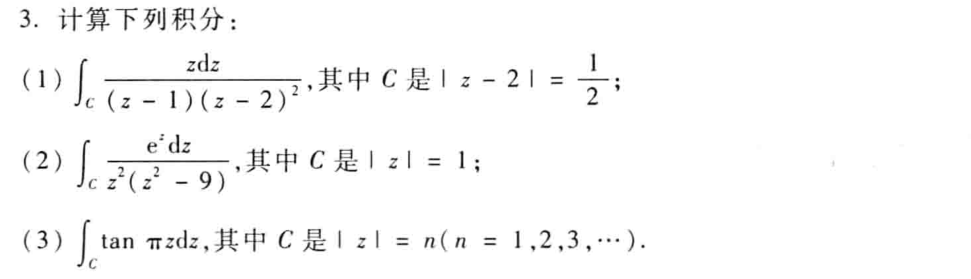
\includegraphics[width=\textwidth]{6-hw9-2025042910.png}
% \caption{}
\label{}
\end{figure}
\end{exercise}
(1)
\[
\begin{aligned}
\int_{C}^{} \frac{z}{(z-1)(z-2)} \, \mathrm{d}z & =2\pi i\cdot \mathrm{res}_{2} \left( \frac{z}{(z-1)(z-2)} \right) \\
 & =2\pi i\cdot \lim_{ z \to 2 } (z-2)\cdot\frac{z}{(z-1)(z-2)} \\
 & =4\pi i
\end{aligned}
\]
(2)
\[
\begin{aligned}
\int_{C}^{} \frac{e^{ z }}{z^2(z^2-9)} \, \mathrm{d}z  & =2\pi i\cdot \mathrm{res}_{0}\left( \frac{e^{ z }}{z^2(z^2-9)} \right) \\
 & =2\pi i\cdot \lim_{ z \to 0 } \frac{\mathrm{d}}{\mathrm{d}z} \left[ z^2\cdot\frac{e^{ z }}{z^2(z^2-9)} \right] \\
 & =2\pi i \cdot\left( -\frac{1}{9} \right) \\
 & =-\frac{2}{9}\pi i
\end{aligned}
\]
(3)
\[
\begin{aligned}
\int_{C}^{} \tan \pi z \, \mathrm{d}z & =2\pi i\cdot \sum_{j=-n+1}^{n} \mathrm{res}_{j-\frac{1}{2}}(\tan \pi z) \\
 & =2\pi i\cdot \sum_{j=-n+1}^{n} \lim_{ z \to j-\frac{1}{2} } \left( z-j+\frac{1}{2} \right)\cdot\frac{\sin \pi z}{\cos \pi z} \\
 & =2\pi i\sum_{j=-n+1}^{n} -\frac{1}{\pi}  \\
 & =-4ni
\end{aligned}
\]
\begin{exercise}
\begin{figure}[H]
\centering

\includegraphics[width=\textwidth]{7-hw9-2025042910.png}
% \caption{}
\label{}
\end{figure}
\end{exercise}
记奇点为 $z_1,z_2,\dots,z_n$,我们知道
\[
2\pi i \sum_{j=1}^{n}\mathrm{res}_{z_j}f(z)=-2\pi i\cdot\mathrm{res}_{_{\infty}}f(z)
\]
由于 $f$ 在 $z=\infty$ 处解析,所以 $\mathrm{res}_{\infty}f(z)=0$. 从而
\[
\sum_{j=1}^{n} \mathrm{res}_{z_j}f(z)=0
\]
记
\[
f(z)=\frac{1}{(z^{5}-1)(z-3)}
\]
在扩充复平面上解析,因为洛朗展开没有正项,所以
\[
\sum_{n=1}^{5} \mathrm{res}_{e^{ i\cdot2n\pi /5 }}f(z)=-\mathrm{res}_{3}f(z)=-\lim_{ z \to 3 } (z-3)f(z)=-\frac{1}{242}
\]
因此
\[
\frac{1}{2\pi i}\int_{\lvert z \rvert =2}^{} f(z) \, \mathrm{d}z =-\frac{1}{242} 
\]